\chapter{Processing and Methodologies}

\section{Processing Flow}
\paragraph{Processing Chart}
\begin{figure}[ht!]
\centering
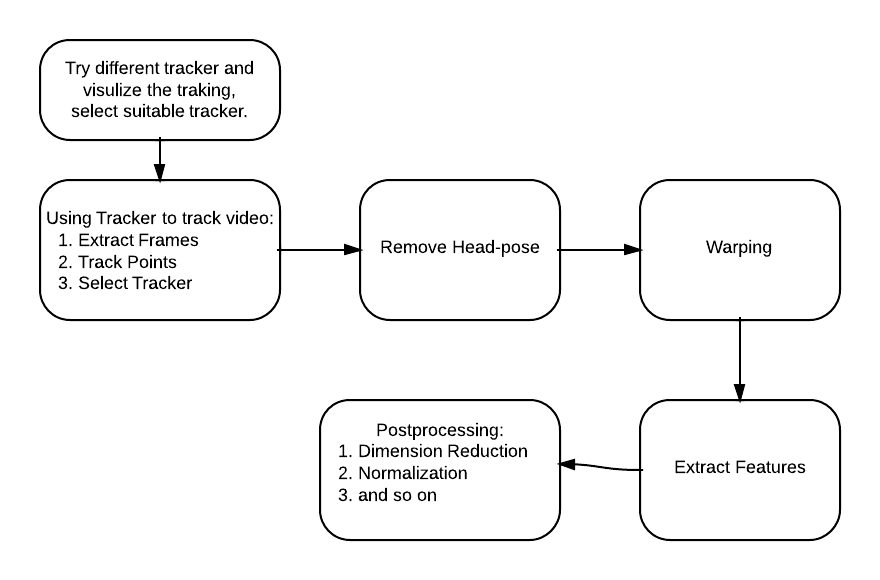
\includegraphics[width=150mm]{imgs/ProcedureChart.png}
\caption{Main procedures}
\end{figure}
The figure above shows main procedure of the whole project. At beginning, I tried several trackers. Intraface and DRMF are two trackers I tried and compared most. Two trackers are using different methods and also implemented in different languages. Intraface are programmed in c and matlab and has great interface for matlab. I tried two version of DRMF, DRMF programmed using CUDA which uses parallel processing is quite fast. As the programme of DRMF doesn't integrate extract frames from videos. The images are extracted using external function, then tracked using DRMF. I choose Intraface as the final choose, the reason and comparison will be given in later section. Remove head-pose seems to be a very important part for this project, as subject's head moves frequently in many videos. After having tracking points without head-pose, each face in each frame is warped and scaled to same size grey image. Extracting features is to extract appearance feature of each face in the image. Post-processing is preprocessing before using the data for classification.
\paragraph{Data flow Chart}
\begin{figure}[ht!]
\centering
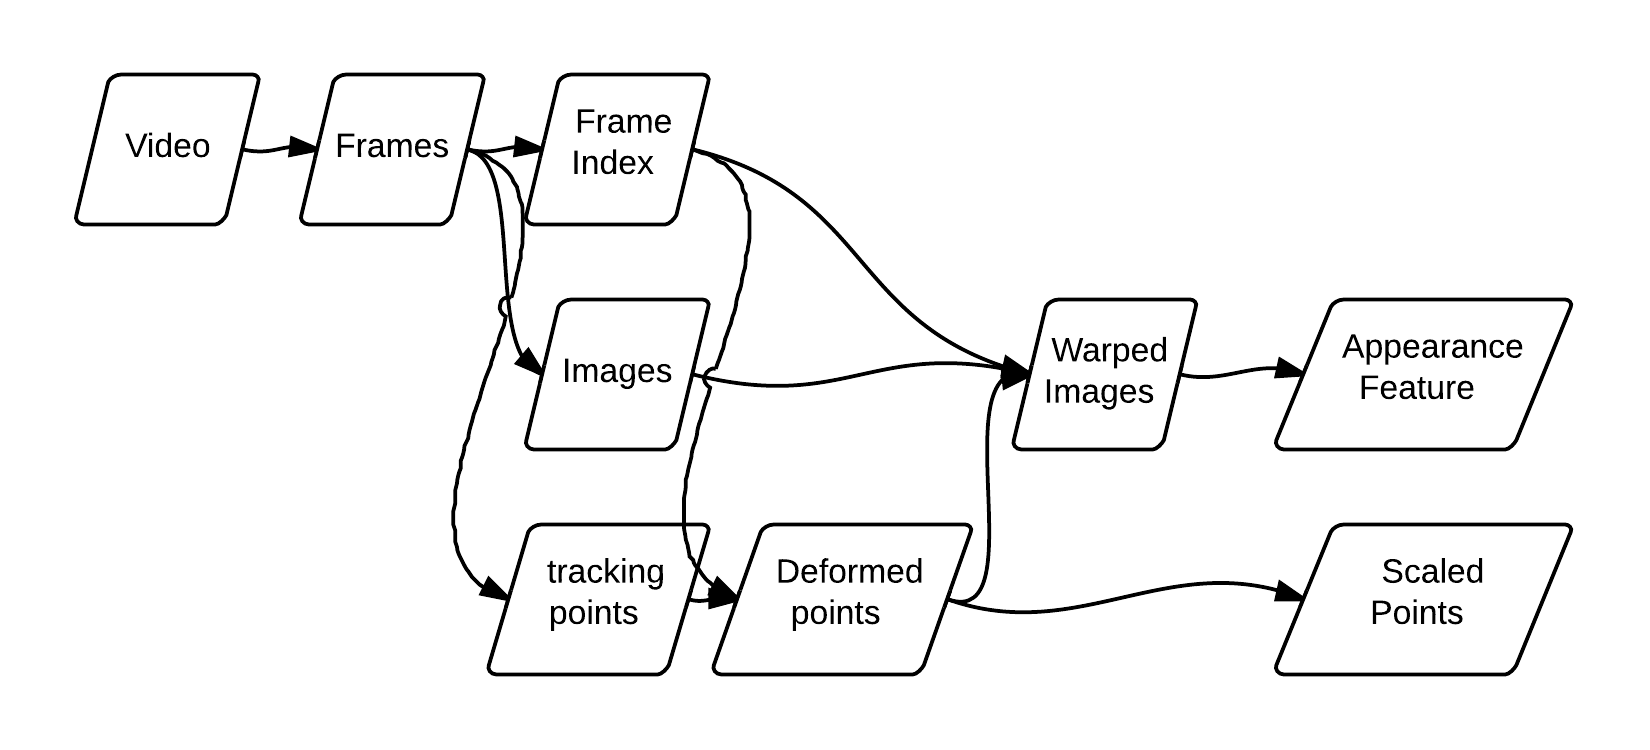
\includegraphics[width=150mm]{imgs/DataFlowChart.png}
\caption{Eating sequence tracked by Intraface}
\end{figure}

There are two types of encoded video, one is in format of fly and the other is avi. Extracting frames from videos is proceed with Intraface and stored in formats of jpeg and mat which used for processing of matlab. There are several situations that a track is unable to track a face in the image such as no subject in the image, the head is face to a very large angle from frontal face, face is partially not show in the frame. Frame index points to those images which the tracker is able to tracker a face in a frame. Image is the frame images stored in mat format. Different tracker may tracks different number of characteristic facial points. Intraface tracks 49 facial points and DRMF tracks 66 points. Deformed points is the tracking point after removed head-pose. Warped Images is the face after remove head-pose and background which only leaves the meshes build by tracking points. Appearance feature is face feature extracted using local binary pattern (LBP). As the image size from image to warped images are changed, the points is rescaled from deformed point to scaled points.

\section{Face Alignment}
Face alignment is to align face in one image with respect to the same face in another image. Face alignment techniques are used to track characteristic facial points in image sequences. In this project, the aim of face alignment is to localise the feature points on face images. The points are usually around eyes, nose, mouth, and outline. Face alignment techniques are essential on face recognition, modelling and synthesis. There are three main different approaches Parametrized Appearance Models(PAMs), Discriminative approaches, Part-based deformable models. Parametrized appearance models contains many models such as active appearance models (AAMs), morphrable models, eigentrackings, and template tracking \cite{xiong2013supervised}. All these models are using PCA method to parametrize a face. A face could approximately decomposed as linear combination of shape basis and appearance basis. The problem of face alignment could be refer as minimising the difference between the constructed PAM and the face. Common approach is use Gauss-Newton methods \cite{xiong2013supervised}. Discriminative approaches are to learn the linear regression between the head move and appearance change. Part-based deformable model perform face alignment by maximising the posterior likelihood of part locations given image\cite{xiong2013supervised}.

\subsection{Aative Appearance Model}

Active Appearance Model (AAMs) is defined as a generative model of a certain visual phenomenon in \cite{matthews2004active}. AAMs are conceptually related to morphable models, constrained models and active blobs. In this project, it is refer to a model of face. As AAM is conceptually related to other parameterized appearance model, so it is introduced as an example of parameterized appearance model for understanding purpose. According to \cite{matthews2004active}, there are two types of AAMs, one refers as independent shape and appearance models, which model shape and appearance independently, and the other refers as combined shape and appearance models, which parameterized shape and appearance model with a single set of linear parameters \cite{matthews2004active}. Normally AAMs appears along with a fitting algorithm. However, in the following context, it only refers to a model.\cite{matthews2004active} gave a well explain about what is an AAM, most of following theory are from \cite{matthews2004active}. \newline
\paragraph{Shape}
Shape of a face $s$ is defined by coordinates $(x,y)$ of $v$ vectices of face points and the mesh they built:
\begin{equation}
s = (x_{1},y_{1},x_{2},y_{2},...,x_{v},y_{v})^{T}
\end{equation}
\newline
$s$ also can be expressed as a base shape $s_{0}$ plus linear combination of $n$ shape vectors $s_{i}$:
\begin{equation}
s = s_{i} + \sum_{i =1}^{n}p_{i}s_{i}
\end{equation}
\newline
\paragraph{Appearance}
For all pixels x in the mesh $s_{0}$, appearance $A(0)$ can be expressed by base appearance $A_{0}(x)$ and m appearance images $A_{i}(x)$.
\begin{equation}
A(x) = A_{0}(x) + \sum_{i=1}^{m}\lambda_{i}A_{i}(x) \qquad \forall x \in s_{0}
\end{equation}
\newline
AAMs are usually computed by applying Principle Component Analysis (PCA) to choosen images. The chosen images contains a variety of shapes. The base shape $s_{0}$ is the mean shape and the vector $s_{v}$ is the eigenvector corresponding to the largest $v$ eigenvalues. The base appearance $A_{0}$ and the appearance $A_{i}$ is computed by applying Principle Component Analysis to a set of shape normalised images.
\paragraph{Model} 
$W(x:p)$ is the warp from $s_{0}$ to $s$. Then the model $M$ set the appearance of $W(x:p)$ to $A(x)$.
\begin{equation}
M(W(x:p)) = A(x)
\end{equation}
\newline
Combined AAMs
\newline
Combined AAMs just use parameter $c = (c_{1},c_{2},...)^{T}$ to parametrize shape:
\begin{equation}
s = s_{0} + \sum_{i=1}^{l}c_{i}s_{i}
\end{equation}
and appearance:
\begin{equation}
A(x) = A_{0}(x) + \sum_{i=1}^{l}c_{i}A_{i}(x)
\end{equation}

\subsection{Trackers}
In the processing of face alignment I tried three trackers, but mainly using two trackers, one is from Intraface \cite{xiong2013supervised} and the other DRMF \cite{asthana2013robust}. 
\paragraph{Intraface}
\cite{xiong2013supervised} implies image alignment  can be posed as solving a nonlinear optimization problem. It uses Supervised Descent Method for minimising Non-linear Least Square(NLS) function, which avoids calculating the Hessian and the Jacobian that could be computationally expensive.
\newline
Examples:
\begin{figure}[ht!]
\centering
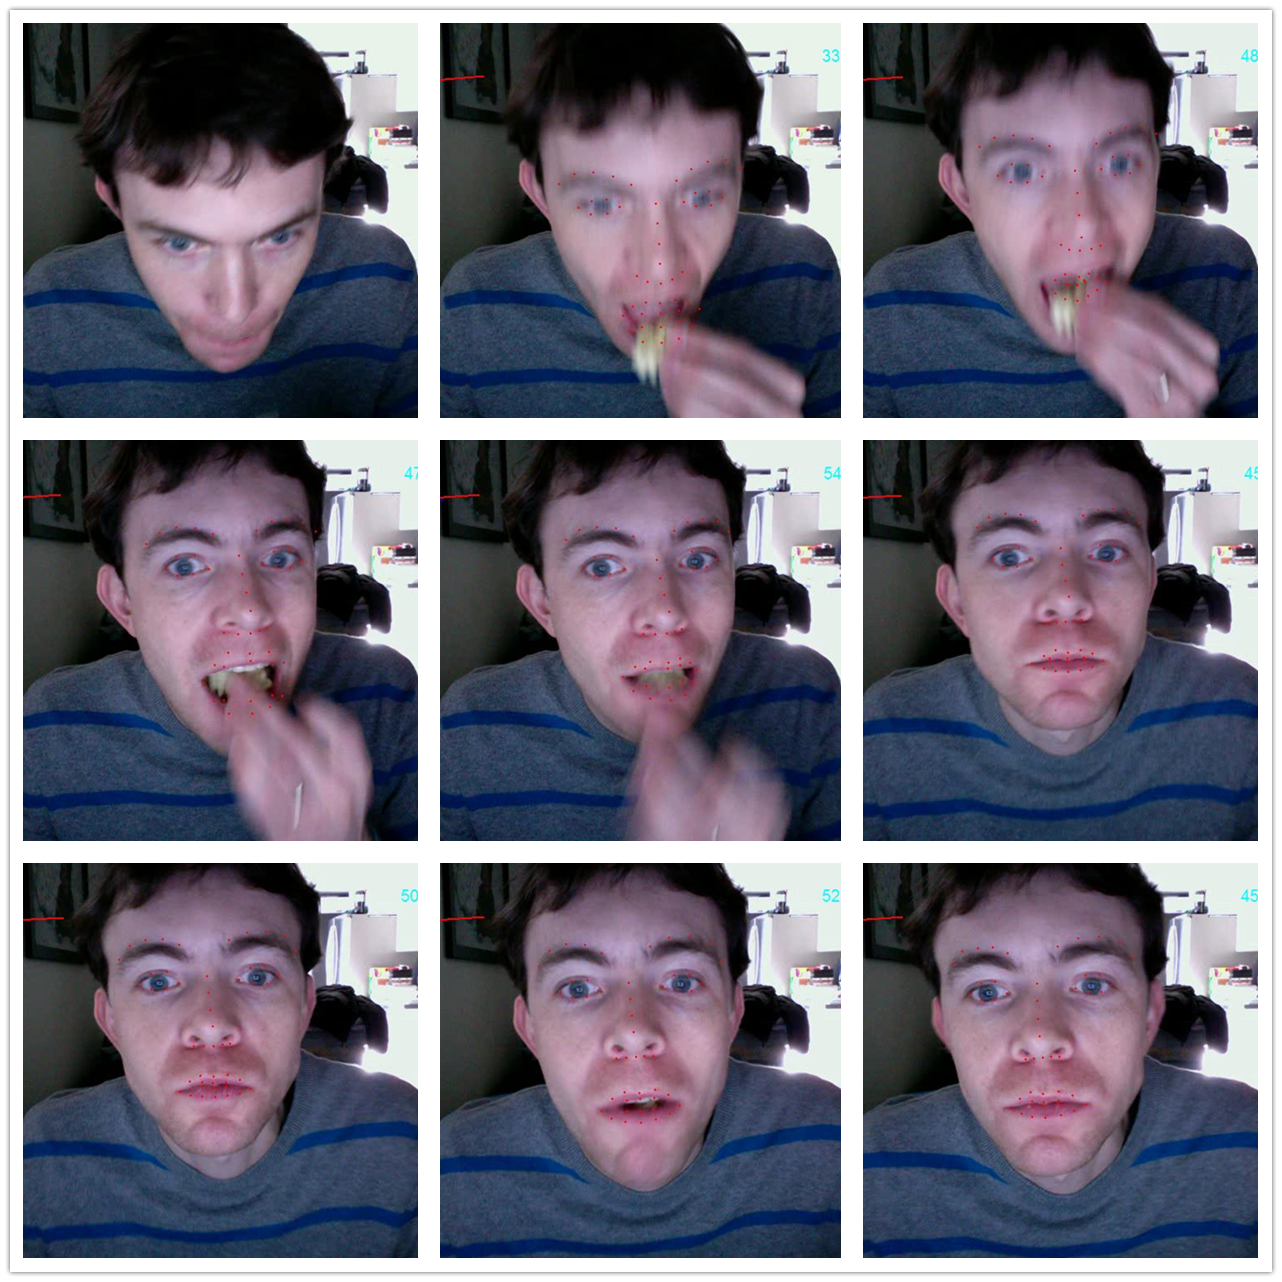
\includegraphics[width=90mm]{imgs/Tracking_Intraface_eating_red.png}
\caption{Eating sequence tracked by Intraface}
\end{figure}

\begin{figure}[ht!]
\centering
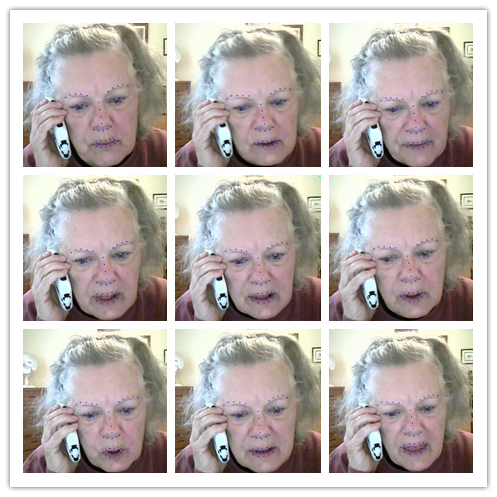
\includegraphics[width=90mm]{imgs/Talking_Intraface_140711_176_184.png}
\caption{Talking sequence tracked by Intraface}
\end{figure}

\paragraph{DRMF}
DRMF uses novel discriminative regression based on Constrained Local Models(CLMs) for face alignment.
\newline
Examples:
\begin{figure}[ht!]
\centering
\includegraphics[width=90mm]{imgs/Talking_DRMF_140711_176_184.png}
\caption{Talking sequence tracked by DRMF}
\end{figure}

\begin{figure}[ht!]
\centering
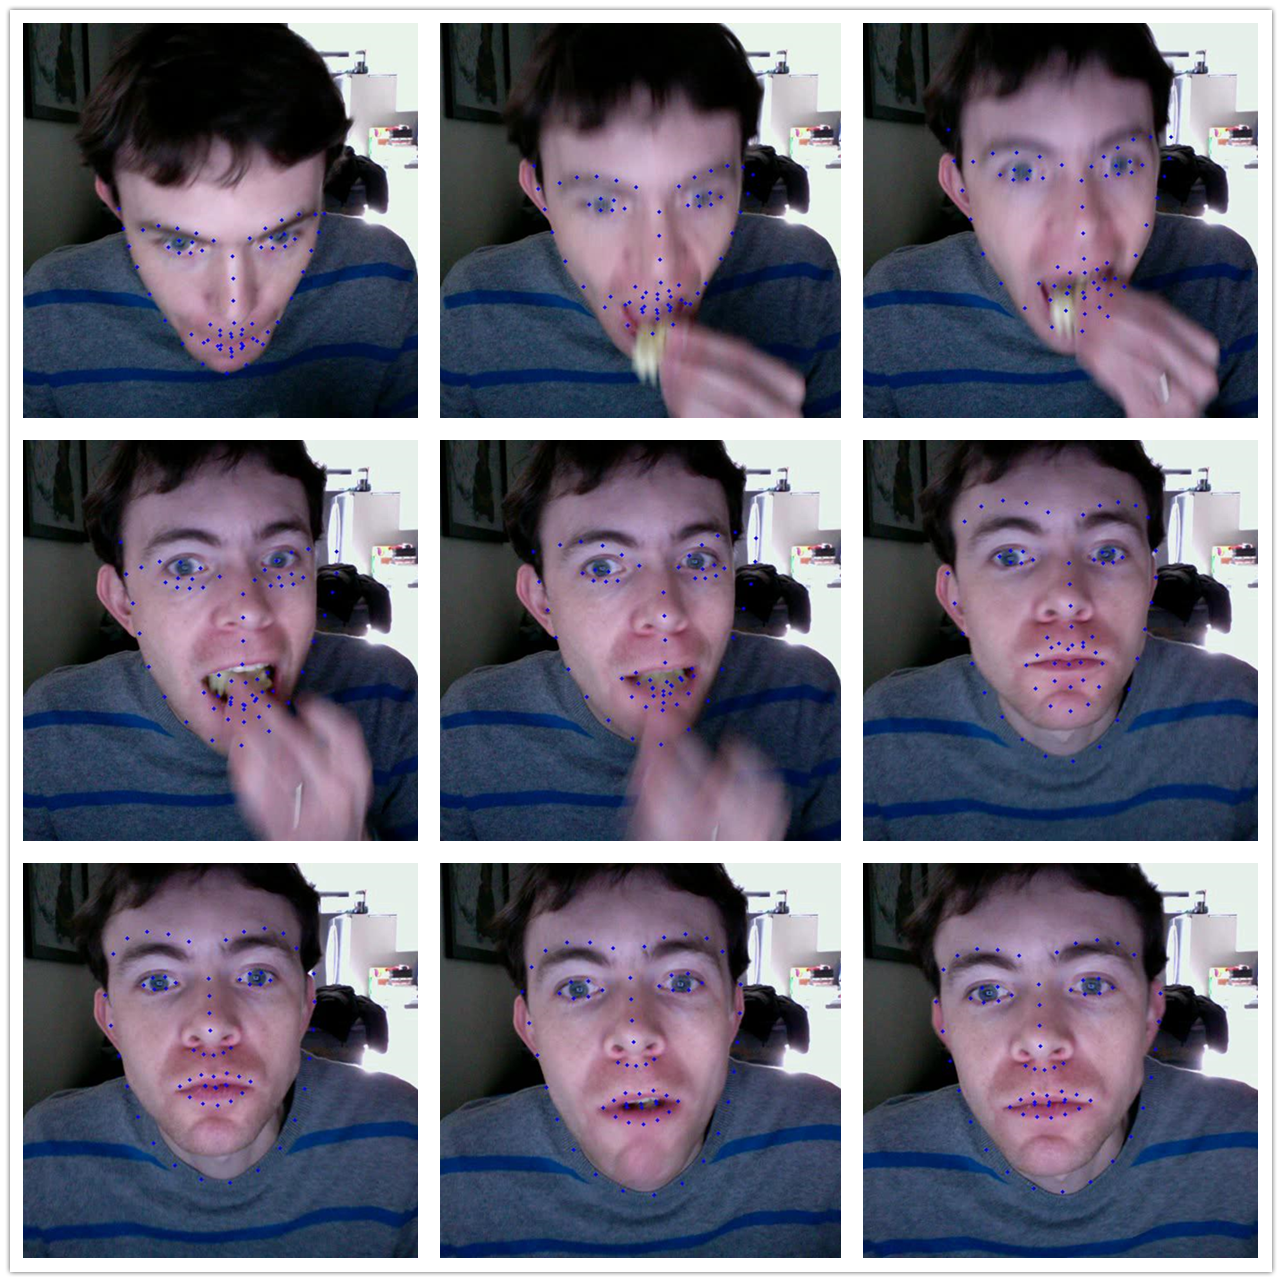
\includegraphics[width=90mm]{imgs/Tracking_DRMF_eating.png}
\caption{Eating sequence tracked by DRMF}
\end{figure}


\subsection{Comparison}
\cite{xiong2013supervised} implies that face alignment problem are usually treated as  solving continuous nonlinear optimisation problem. \cite{xiong2013supervised} uses supervised descent method (SDM) for minimising the  Non-linear Least Square (NLS) function. \cite{asthana2013robust} uses discriminative regression approach for constrained local method (CLM). However, from the computing time and alignment results, \cite{xiong2013supervised} is better than \cite{asthana2013robust} in many aspects.
\newline

\begin{figure}[ht!]
\centering
\includegraphics[width=90mm]{imgs/Tracking_Intraface_DRMF_compare_00.png}
\caption{Talking sequence tracked by DRMF}
\end{figure}

\begin{figure}[ht!]
\centering
\includegraphics[width=90mm]{imgs/Tracking_Intraface_DRMF_comparison.png}
\caption{Talking sequence tracked by DRMF}
\end{figure}

Description
\section{Remove Head-pose}
The algroithm of removing head-pose from tracking points is in \cite{saragih2011deformable}.The following are some example of orginal track points and deformed points:

\begin{figure}[ht!]
\centering
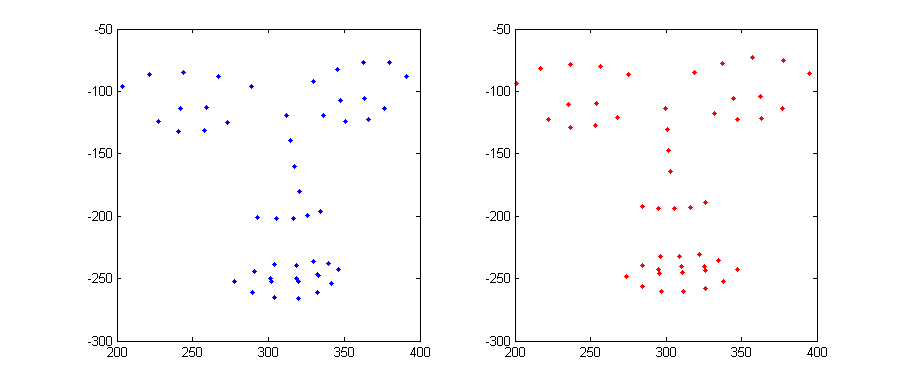
\includegraphics[width=90mm]{imgs/160954_Deform_213.png}
\caption{Talking sequence tracked by DRMF}
\end{figure}

\begin{figure}[ht!]
\centering
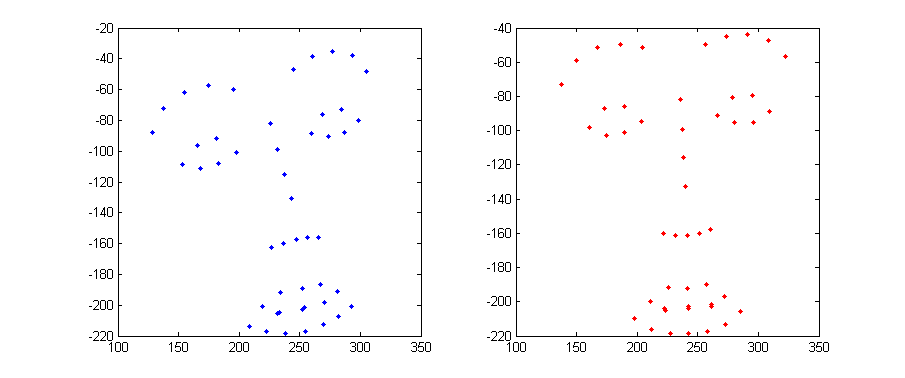
\includegraphics[width=90mm]{imgs/160954_Deform_233.png}
\caption{Talking sequence tracked by DRMF}
\end{figure}

\section{Warping}
In order to have the appearance image of the face after removed head-pose, it is necessary to warp the face with head pose. Basic idea is to for each triangles builded by tracking points, the image points in the triagnles are projected to the corresponding triagnles built by deformed points. The following are some examples of face before and after warping:

\begin{figure}[ht!]
\centering
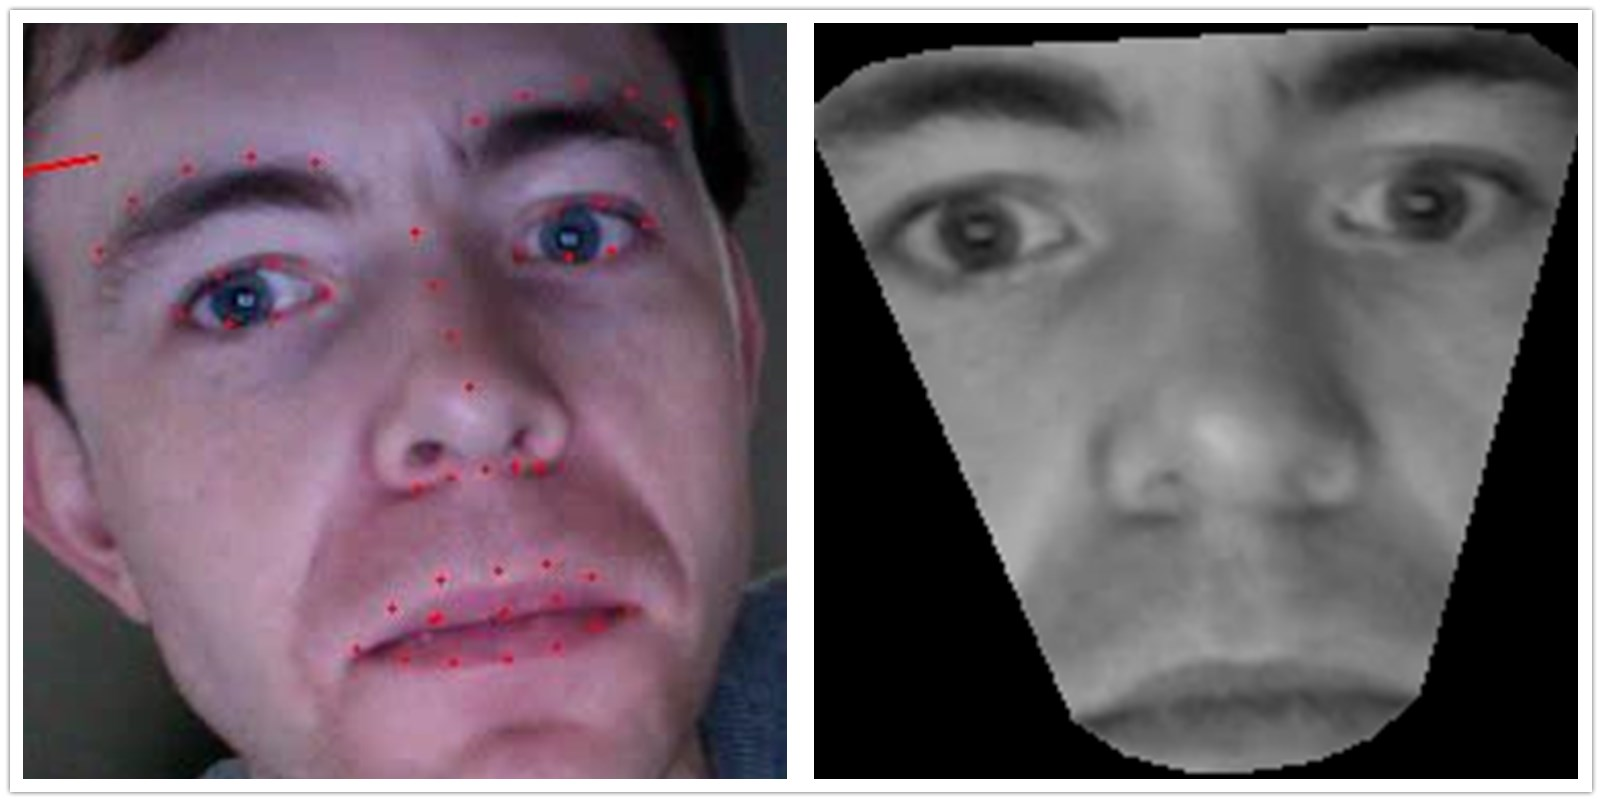
\includegraphics[width=90mm]{imgs/Warping_Intraface_213.png}
\caption{Talking sequence tracked by DRMF}
\end{figure}

\section{Feature Extraction}
The image after warping is not directly used for classfication. The data for classfication is the features of the image. There are many techniques to extract features from images, in this experiment, Local Binary Pattern are used for extracting image feature.
\subsection{Local Binary Pattern}
Effective facial representation of the original face iamges is an important part of successful facial expression recognition.
\section{Postprocessing}
Due to the time limits, in the experiment part, we only use support vector machine to do classfication.
\paragraph{Normalization}

\paragraph{Scaling}